\section{Timing layers for single particles}

Now we discuss the kinematic regions  relevant for  TOF measurements of SM and BSM particles. Instead of the full {\sc geant}4 simulations, we will
use a semi-analytic approach.  
 
To estimate the separation power between different mass hypotheses, we calculate the mass and momentum for which one can achieve a separation 
 significance higher than $3\sigma$ (or p-value$<0.3$\%). 
If there are two particles with mass $m$ and a reference (fixed) mass $m_F$, respectively, the $3\sigma$ separation can be 
achieved for this condition~\cite{Cerri:2018rkm}:
\begin{equation}
\frac{L}{c \sigma_{\textsc{TOF}}}\left|\sqrt{1+\frac{m^2}{p^2}} - \sqrt{1+\frac{m_F^2}{p^2}}\right| > 3
\label{eqTOF}
\end{equation}
where $p$ is the momentum of a particle with mass $m$, $L$  is the length of the particle's trajectory, 
and $\sigma_{TOF}$ is the
resolution  of the timing layer that measures the TOF.

Figure~\ref{fig:singleparticles} shows the $3\sigma$ separation from the pion
mass hypothesis ($m_F=m_{\pi}$) using the procedure discussed  in~\cite{Cerri:2018rkm}. The 
calculations are performed for several values of resolution of the timing layer, ranging from 10~ps to 1~ns,
as a function of $L$ and $p$. For a 20~ps detector and a typical travel 
distance $L\sim 1.5-2$~m from the production vertex to the ECAL, neutrons and protons can be separated from the pion hypothesis up to $p \approx 7$~GeV. 
The separation of kaons from pions can be performed up to 3~GeV.
This momentum range should be sufficient for a reliable particle 
identification in a momentum range adequate for some physics studies focused on
single-particle reconstruction (such as B-meson physics).
This can also be used for jets that are dominated
by particles in this momentum range.
For a detector  with 1~ns resolution, the separation can only be possible  up to  300 -- 500~MeV. This is smaller than the 
minimum particle momentum of $\approx$0.5~GeV considered for high-energy proton colliders.
Therefore, a timing layer with 1~ns resolution cannot be used for particle identification in such experiments.

\begin{figure}
\begin{center}
   \subfigure[Neutrons] {
   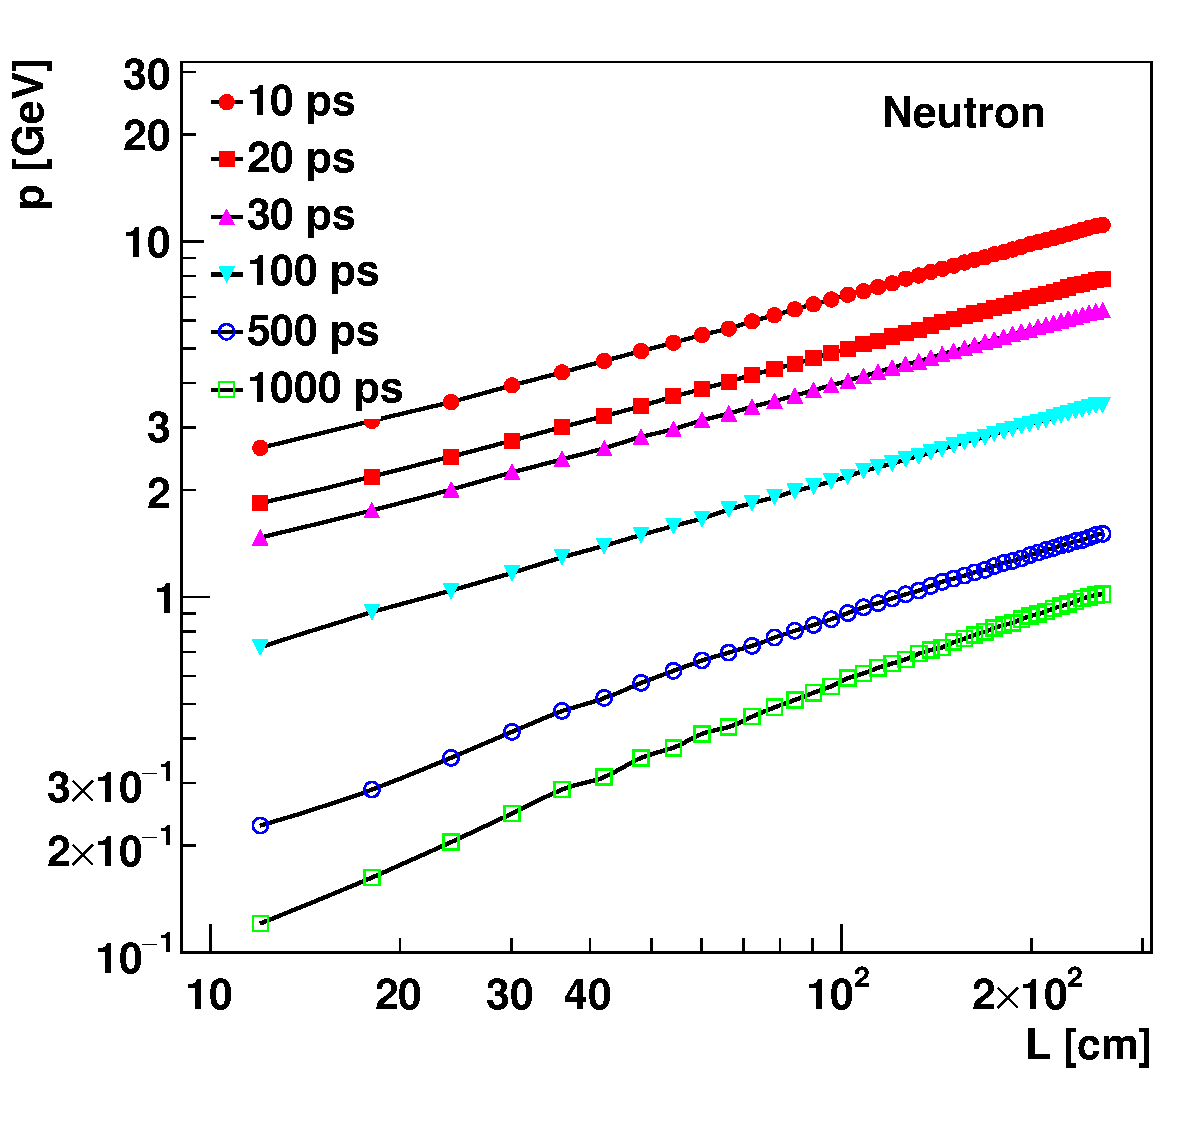
\includegraphics[width=0.45\textwidth]{time_flight_length_neutron.pdf}
   }
      \subfigure[$K$-mesons] {
   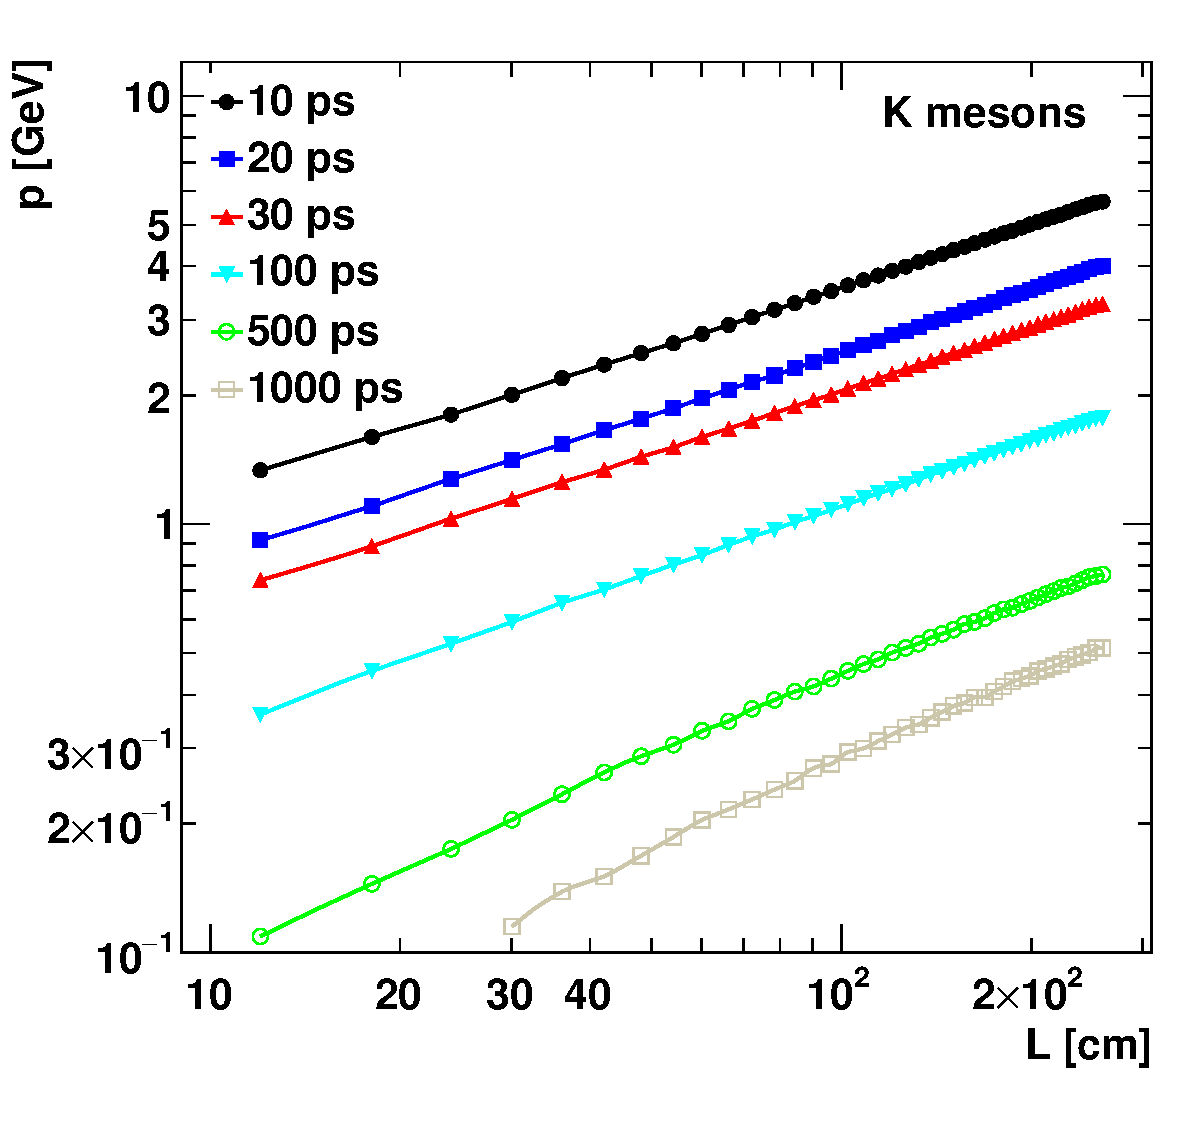
\includegraphics[width=0.45\textwidth]{time_flight_length_kion.pdf}\hfill
   }
\end{center}
\caption{
The $3\sigma$ separation from the pion-mass hypothesis for (a) neutrons and (b) kaons as a function of the length of the particle's trajectory $L$ 
and the momentum $p$. The lines show extrapolated results between the calculations indicated by the symbols.  
}
\label{fig:singleparticles}
\end{figure}


\begin{figure}
\begin{center}
   \subfigure[for $L=2$~m] {
   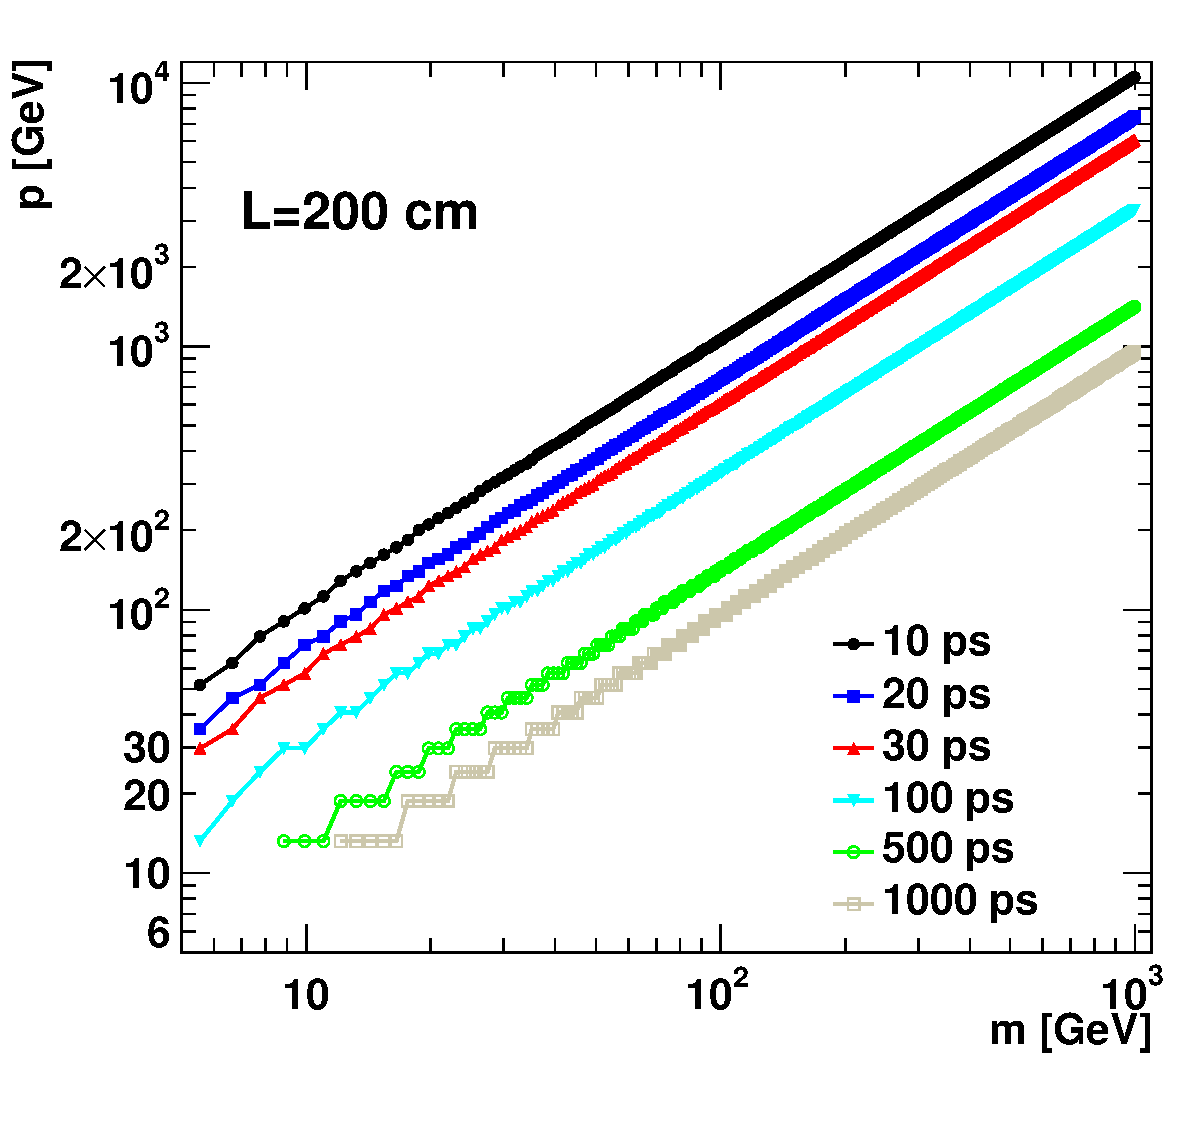
\includegraphics[width=0.45\textwidth]{time_flight_200.pdf}
   }
   \subfigure[for $L=0.2$~m] {
   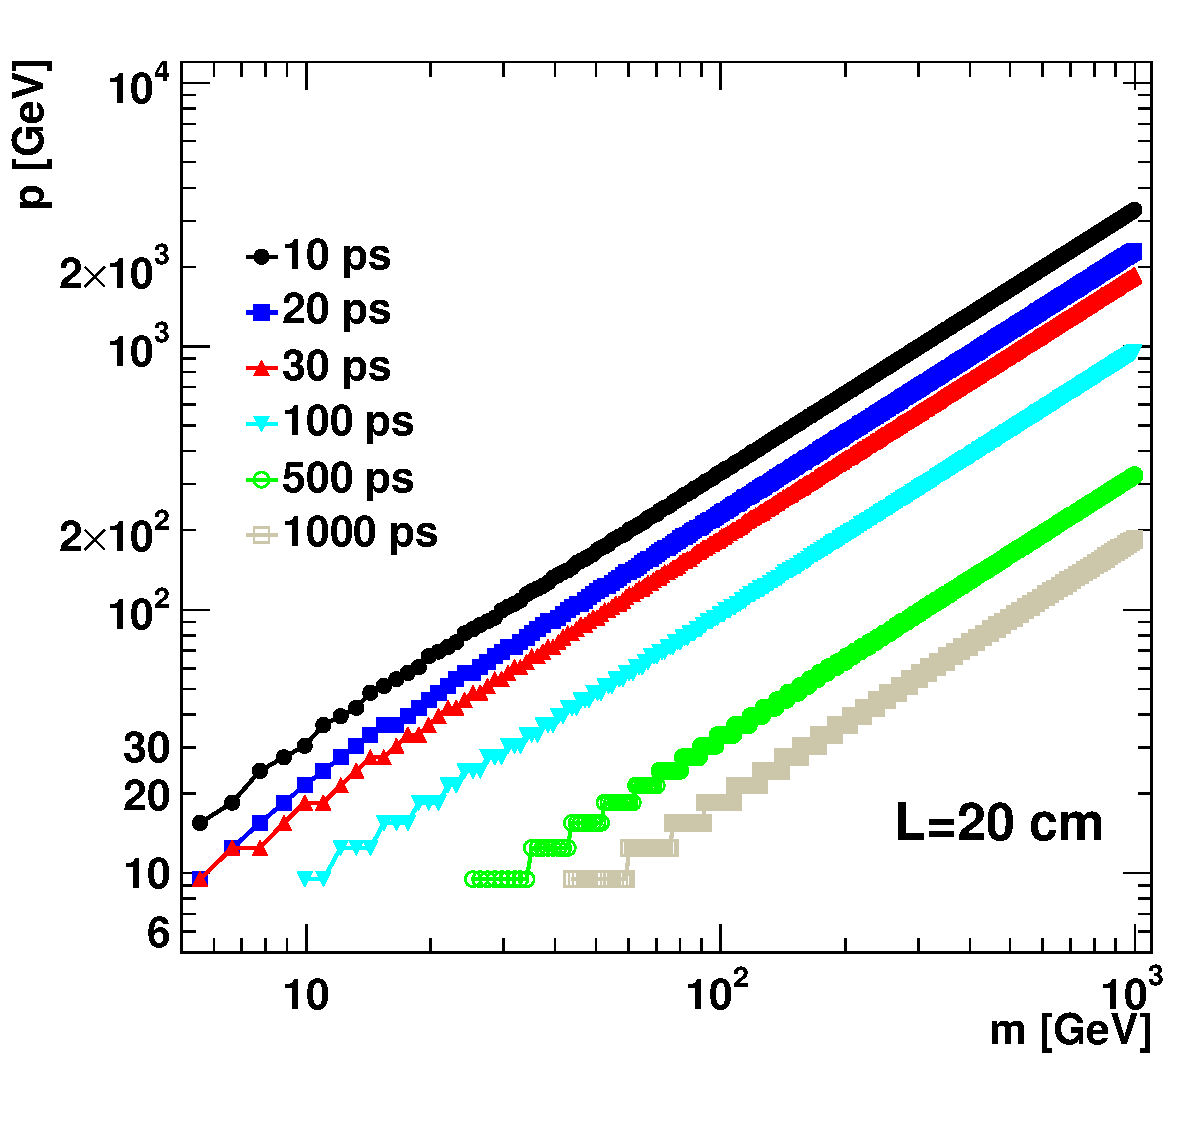
\includegraphics[width=0.45\textwidth]{time_flight_20.pdf}\hfill
   }
\end{center}
\caption{
The $3\sigma$ separation between heavy particles and $\alpha$ particles assuming timing layers with different resolutions for TOF, and using (a) $L=2$~m and (b) $L=0.2$~m.
The first value of $L$ is the typical distance
from the interaction vertex to the first layer TL1, while the second value is the typical  distance
between the two timing layers enclosing an ECAL based on the silicon technology.
}
\label{fig:signgleBSM}
\end{figure}

Having discussed the rather classical cases of discriminating  neutrons, protons and kaons from the pion hypothesis,
let us turn to the BSM searches for heavy particles.
The largest SM  backgrounds for light BSM  particles are primary protons and neutrons.
Other stable particles that can be produced by secondary interactions in the 
detector material or the beam pipe are deuterons and $\alpha$ particles. 
Although the $\alpha$ particle rate is  low since they stop easily in detector material,
it may still represent background for rare BSM particle searches.  
Therefore, we choose  $m_F=m_{\alpha}\simeq 3.73$~GeV  as reference\footnote{We clarify that the choice of $\alpha$ particles as the reference mass is
arbitrary and is only motivated by our attempt to check the $3\sigma$ separation in the momentum range $p<10$~GeV.} in  Eq.~\ref{eqTOF}, and evaluate the
$3\sigma$ separation for a wide range of masses and momenta above 4~GeV.
For many planned experiments the distance between the $pp$ collision point and the first layer of the ECAL is 
$1.5-2.5$~m. Therefore we use $L=2$~m and consider 0.2~m as the separation between the TL2 and TL1 timing layers.

Figure~\ref{fig:signgleBSM} shows the discrimination power for different choices of the timing layer resolution
and the distance $L$ (see Fig.~\ref{fig:eff_rad}).
For $L=2$~m, a stable heavy particle of mass 100~GeV can be discriminated for momentum up to 
700~GeV assuming a 20-ps timing layer,
but only up to 50~GeV using the standard 1~ns resolution.

When  TOF is measured between the layers TL1 and TL2, and assuming a spatial match of the hits, the knowledge of the interaction vertex is not required.
This type of measurement can be beneficial for neutral particles in events with large pile-up (multiple $pp$ collisions).
The identification power when $L=0.2$~m, i.e. the distance between TL2 and TL1, is shown in Fig.~\ref{fig:signgleBSM}(b).
For a stable particle with mass 100~GeV, the identification is possible up to about 200~GeV in momentum. The standard calorimeter with
1~ns resolution can only perform the identification up to $20$~GeV. 
